\documentclass[11pt]{article}
\usepackage[french, english]{babel}
\usepackage[utf8]{inputenc}
\usepackage{graphicx}
\usepackage{framed}
\usepackage[normalem]{ulem}
\usepackage{amsmath}
\usepackage{amsthm}
\usepackage{amssymb}
\usepackage{amsfonts}
\usepackage{enumerate}
\usepackage{import}
\usepackage[top=1 in,bottom=1in, left=1 in, right=1 in]{geometry}
\usepackage{listingsutf8}
\usepackage{color}
\usepackage{float}
\usepackage{graphicx}
\usepackage{subcaption}
\usepackage[toc,page]{appendix}
\floatstyle{boxed} 
\restylefloat{figure}
\definecolor{mygreen}{rgb}{0,0.6,0}
\definecolor{mygray}{rgb}{0.5,0.5,0.5}
\definecolor{mymauve}{rgb}{0.58,0,0.82}
\newcommand{\dt}{\partial_t}
\newcommand{\Tl}{\frac{T}{\lambda}}
\theoremstyle{definition}
\newtheorem{definition}{Définition}[section]
 


\lstset{ 
  backgroundcolor=\color{white},   % choose the background color; you must add \usepackage{color} or \usepackage{xcolor}; should come as last argument
  basicstyle=\footnotesize,        % the size of the fonts that are used for the code
  breakatwhitespace=false,         % sets if automatic breaks should only happen at whitespace
  breaklines=true,                 % sets automatic line breaking
  captionpos=b,                    % sets the caption-position to bottom
  commentstyle=\color{mygreen},    % comment style
  deletekeywords={...},            % if you want to delete keywords from the given language
  escapeinside={\%*}{*)},          % if you want to add LaTeX within your code
  extendedchars=true,              % lets you use non-ASCII characters; for 8-bits encodings only, does not work with UTF-8
  firstnumber=1000,                % start line enumeration with line 1000
  frame=single,	                   % adds a frame around the code
  keepspaces=true,                 % keeps spaces in text, useful for keeping indentation of code (possibly needs columns=flexible)
  keywordstyle=\color{blue},       % keyword style
  language=Python,                 % the language of the code
  morekeywords={*,...},            % if you want to add more keywords to the set
  numbers=left,                    % where to put the line-numbers; possible values are (none, left, right)
  numbersep=5pt,                   % how far the line-numbers are from the code
  numberstyle=\tiny\color{mygray}, % the style that is used for the line-numbers
  rulecolor=\color{black},         % if not set, the frame-color may be changed on line-breaks within not-black text (e.g. comments (green here))
  showspaces=false,                % show spaces everywhere adding particular underscores; it overrides 'showstringspaces'
  showstringspaces=false,          % underline spaces within strings only
  showtabs=false,                  % show tabs within strings adding particular underscores
  stepnumber=2,                    % the step between two line-numbers. If it's 1, each line will be numbered
  stringstyle=\color{mymauve},     % string literal style
  tabsize=2,	                   % sets default tabsize to 2 spaces
  title=\lstname                   % show the filename of files included with \lstinputlisting; also try caption instead of title
}
\lstset{inputencoding=utf8/latin1}
\newcommand{\Dt}{\Delta t}
\newcommand{\Dx}{\Delta x}

\title{\textbf{Dynamique de réseaux multi-échelles complexes sous contraintes: Modélisation et Analyse}}
\author{Liam Toran}
\date{}
\begin{document}
\selectlanguage{french}
\maketitle
\vspace{-20px}
\begin{center}
Stage de fin de M2A 2019 au Laboratoire J.A. Dieudonné de l'Université de Nice\\ sous la supervision de Yves D'Angelo, Rémi Catellier, Laurent Monasse
\end{center}
{\footnotesize Thèmes: Mathématiques et leurs Interactions, Modélisation, Analyse, Processus Stochastiques, Équations aux dérivées partielles et ordinaires, Stabilité, Réaction-Diffusion, Ondes progressives, Simulation Numérique.}
\begin{figure}[hb]
\begin{subfigure}[b]{0.5\textwidth}
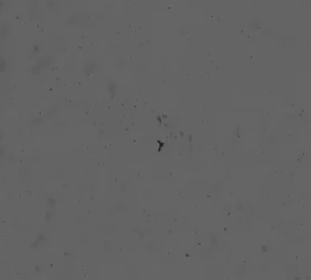
\includegraphics[width=\textwidth]{Images/1.png}
\end{subfigure}
\begin{subfigure}[b]{0.5\textwidth}
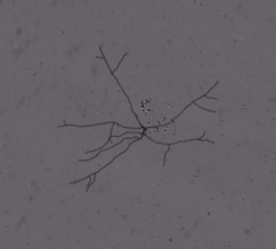
\includegraphics[width=\textwidth]{Images/2.png}
\end{subfigure}
\begin{subfigure}[b]{0.5\textwidth}
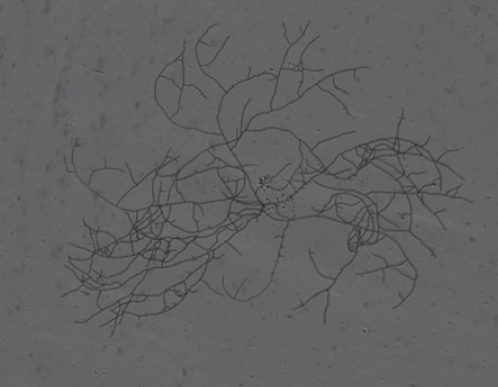
\includegraphics[width=\textwidth]{Images/3.png}
\end{subfigure}
\begin{subfigure}[b]{0.5\textwidth}
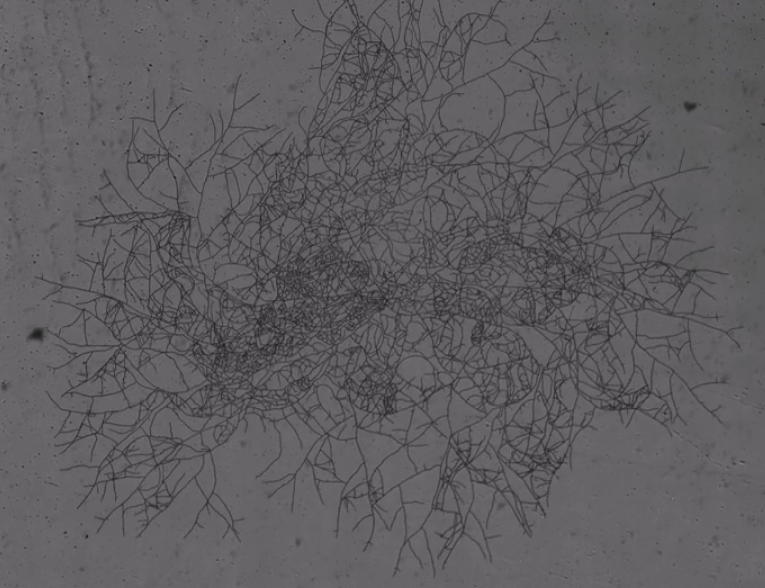
\includegraphics[width=\textwidth]{Images/4.png}
\end{subfigure}
\caption{Capture d'un réseau de champignon en expension, par}
\end{figure}
\newpage
\tableofcontents
\newpage



\section{L'équation de Fisher ou KPP}
\subsection{Préliminaire}
Notre point de départ est l'équation de diffusion:\begin{equation}\dt u = \Delta u  \end{equation}
En plus de la diffusion, considérons des modèles où le taux d'accroissement de $u$ dépend aussi de la densité $u$.\\
Ceci donne les équations de reaction-diffusion:
\begin{equation}\dt u = \Delta u + F(u) \label{eq:ReaDi} \end{equation} 
où F est assez lisse.\\
Il est souvent naturel dans les modèles de considérer $F(u)$ proportionnel à  $u$ pour $u$ petit (``croissance"), et quand $u$ devient proche de 1, l'accroissement $F(u)$ s'arrête: $F(1)=0$ (``saturation").\\
Ces types de modèles ont étés introduits et examinés par les travaux de Fisher[1] %CITER FISHER
et Kolmogorov, Petrovsky et Piscounuv (abrégés KPP).\\ %CITER KPP
Un exemple d'une telle équation est:

\begin{equation}
	\dt u = \Delta u + ru(1-u) \label{eq:KPP}
\end{equation}
où $r>0$, qui sera dans la suite étudiée dans le cas 1-dimensionnel en $x$ : $u=u(x,t)$.

\subsection{Réaction}
En observant les solutions constantes en $x$: $u(x,t)=v(t)$ dans \eqref{eq:KPP}, l'équation différentielle ordinaire (EDO ou ODE): \begin{equation}
	\dt v = r(v - v^2) = F(v)
\end{equation}
est obtenue. \\
Il y a deux équilibres ($F(v)=0)$) pour $v=0$ et $v=1$.Par le théorème de stabilité de Lyapunov, $F'(0)>0$ montre que $v=0$ est instable et $F'(1)<0$ montre $v=1$ est asymptotiquement stable.

\subsection{Réaction-Diffusion}
Dans l’espace $X=C^0_{b,unif}(\mathbb{R},\mathbb{R})$ des fonctions bornées et uniformément continues, il y a existence locale et unicité des solutions de l’équation de Fisher-KPP \eqref{eq:ReaDi}. Grâce à un principe du maximum, il y a aussi existence globale et unicité des solutions.
\newtheorem{theorem}{Théorème}
\begin{theorem}:\\ Existence et Unicité de la solution dans $X$: Soit $U_0 \in X$. Il existe une unique solution de l'équation de Fisher-KPP \eqref{eq:ReaDi}  $U \in C([0,\infty[,X)$ avec condition initiale $U_0$. \end{theorem}
\begin{theorem}:\\ Principe du Maximum: Soit $u_1$ et $u_2$ deux solutions de \eqref{eq:ReaDi}. Si il éxiste $t_0$ tel que $u_1(x,t_0)<u_2(x,t_0) $ $\forall x$ alors $u_1(x,t)<u_2(x,t)$  $ \forall x$ et $\forall t>t_0$ \end{theorem}

\subsection{Solutions en onde plane stationnaire / onde progressive}
Rappellons la définition d'une solution en onde plane stationnaire / onde progressive:
\begin{definition}{Solutions en onde plane stationnaire}\\Une solution en onde plane stationnaire est une solution de la forme $u(x,t)=h(x-st)$ où $c \in \mathbb{R} $.\\ On fera parfois l'abus de notation $u(x,t)=u(x-st)$
\end{definition}
Sous des hypothèses ``faibles" sur $F$, l'équation \eqref{eq:ReaDi}: $\dt u = \Delta u + F(u)$ a alors la propriété surprenante et importante de posséder des solutions en ondes planes stationnaires liant les états d'équilibre $u=1$ (à $-\infty$) et $u=0$ (à $+\infty$).\\
Les hypothèses sur $F$ portent en partie sur le fait que \eqref{eq:ReaDi} doit posséder:\\
- Deux états d'équilibre $u=1$ et $u=0$: $F(0)=F(1)=0$:\\
- Un phénomène de ``croissance" : $F'(0)>0$\\
- Un phénomène de ``saturation" : $F'(1)<0$ \\
\paragraph{Étude des solutions en ondes progressive de \eqref{eq:ReaDi}}:\\
En substituant $u(x,t) = h(x-st) = h(y)$ pour $y=x-st$ dans \eqref{eq:ReaDi}, les équations obtenues sur $h$ sont: \begin{equation} \label{eq:FWS} \left\{
                \begin{array}{ll}
                h''(y)+ sh'(y)+F(h(y))=0 \\
                h(-\infty)= 1 \\  h(+\infty) =0 
                   \end{array}
              \right.
\end{equation} 
qui est une équation elliptique non linéaire. Le problème est donc de trouver $s$ et $h \in C^2$ tels que le système \eqref{eq:FWS} soit vérifié. Le théorème obtenu est le suivant:



\begin{theorem}{\textbf{Existence de solutions en onde progressive pour les équations de reaction-diffusion}}:\\
Soit $F \in C^1([0,1])$ tel $F(0)=F(1)=0$ et $F\geq 0$. \\
Il existe une vitesse critique $s_*$ telle que $s_*^2 \geq 4F'(0)$ et: \\ \\
- i) $\forall s \geq s_*$, l'équation \eqref{eq:FWS} a une solution $h_s:\mathbb{R} \rightarrow ]0,1[$ de classe $C^3$.\\ Cette solution est unique à translation près. \\
- ii)  $\forall s<s_*$ l'équation \eqref{eq:FWS} n'a pas de solution $h:\mathbb{R} \rightarrow [0,1]$
\end{theorem}
\textbf{Remarques}:\\
 Dans le cas ii) il existe des solutions en ondes planes mais elles ne sont pas confinées dans [0,1] ni dans $\mathbb{R}^+$, ce qui ne fait pas de sens dans une étude de densité de population.\\
 Dans le cas de l'équation de Fisher-KPP, c'est à dire pour $F(u)=r(u - u^2)$, on a $s_*^2 = 4F'(0) = 4r $: la vitesse minimale de propagation est $s^* =2\sqrt r $.


\subsection{Théorèmes de sélection de la vitesse pour KPP}
Le théorème important suivant est du aux travaux de Kolmogorov, Petrovsky et Piscounuv de 1937. C'est l'article et le résultat fondateur de la théorie des ondes planes dans les systèmes de réaction-diffusion. %CITER KPP\\

\begin{theorem}{\textbf{Convergence vers une solution d'onde à vitesse minimale pour les solutions de l'équation de Fisher-KPP avec une donnée initiale à support compact }}\\
Soit $u_0 \to ]0,1[$ une donnée initiale à support compact. 
Soit $u$ la solution de l'équation de Fisher-KPP \eqref{eq:KPP} avec $r=1$ et de donnée initiale $u_0$.
Alors quand $t \to \infty$, $u$ converge uniformément en $x$ vers une solution d'onde $h_{s^*}$ de \eqref{eq:FWS} qui se de déplace à vitesse minimale $s^* =2$ :
\begin{equation*}
\sup_{y \in \mathbb{R}}  |u(y+m(t),t)-h_{s^*}(y)| \to_{t\to \infty} 0
\end{equation*}
où $m(t)= 2t - (3/2)\log (t) + y_0 $.
\end{theorem}
Remarque: La vitesse du front est alors $s(t) = \dt m(t) = 2 - \frac{3}{2t} \to_{t\to \infty} 2 $.
\paragraph{}
Ce résultat à été raffiné par la suite par Uchiyama, Bramson et Lau. Leurs travaux apportent plus d'informations sur comment la vitesse du front se sélectionne en fonction de la donnée initiale, et comment il est possible d'obtenir d'autres vitesses de fronts que la vitesse minimale en fonction de la donnée initiale.
\begin{theorem}{\textbf{Sélection de la vitesse pour les solutions de l'équation de Fisher-KPP en fonction de la donnée initiale}}\\
Si $u_0 \to ]0,1[$ vérifie $\lim\inf_{x\to -\infty} u_0(x) > 0$ et $\int_0^{+\infty} xe^xu_0(x) / dx < \infty$\\
alors il existe $y_0 \in \mathbb{R}$ tel que la solution de \eqref{eq:KPP} avec données initiales $u_0$ vérifie
\begin{equation*}
\sup_{y \in \mathbb{R}}  |u(y+m(t),t)-h_{s^*}(y)| \to_{t\to \infty} 0
\end{equation*}
où $m(t)= 2t - (3/2)\log (t) + y_0 $. 
\end{theorem}
D'autres vitesses peuvent être sélectionnées: Si la donnée initiale vérifie $u_0(x) \approx  e^{-\lambda_-(s)x}$ quand $x \to +\infty$ alors la solution converge vers une onde progressive de vitesse $s$.





\newpage
\section{Dyamique de Réseaux en Croissance}
Dans cette section et par la suite nous étudions le modèle sur la croissance de réseaux dynamiques branchant, par exemple un champignon, proposé par Rémi Catellier, Yves D'Angelo et Cristiano Ricci, avec rescaling adéquat:
\begin{equation}\label{eq:BDNG}  \left\{
                \begin{array}{ll}
                \dt\mu + \nabla(\mu v) = f(C)(\mu + \rho) -\mu\rho \\
                   \dt(\mu v)+\nabla(\mu v\times v) +T\nabla\mu=-\lambda\mu v+\mu\nabla C-\mu v \rho \\
                 \dt\rho=  F(v) \mu \\
                  \dt C = -b\rho C
                \end{array}
              \right.
\end{equation} 
L'inconnue $\mu$ représente la densité des apex du champignon.\\
L'inconnue $\rho$ représente la densité des hyphes/ du réseau.\\
L'inconnue $v$ représente la vitesse des apex.\\
L'inconnue $C$ représente la concentration des nutriments.\\
Les paramètres $T$, $\lambda$ et $b$ sont des scalaires représentants la température, l'amortissement fluide sur la vitesse des apex, et le taux de consommation des nutriments par le réseau.\\
La fonction $f$ indique l'influence de la concentration de nutriments sur la croissance du champignon. Pour avoir un état stationnaire sur la croissance du champignon,$f(0)=0$ et $f(x)/x$ dans $L^1$ proche de 0 sont imposés.\\
La fonction $F$ représente l'inverse du temps moyen passé par les apex dans un point donné, et est donné par l'expression:
\begin{equation}
	F(V)=(\frac{1}{2\pi T})^\frac{d}{2}\int_{\mathbb{R}^d} |v|\exp(-\frac{|v-V|^2}{2T})dv\end{equation}
où d est la dimension du problème. Ceci est souvent simplifié en substituant $F(V)$ par une constante: $F(V)= F_0$ .\\

\subsection{Explication des équations du système \eqref{eq:BDNG}}
Le champignon est un réseau branchant dynamique qui peut être étudié en deux parties: les apex (pointes du réseau) représentés par leur densité $\mu$ et les hyphes (branches du réseau) représentés par leur densité $\rho$\\
Les lignes du système \eqref{eq:BDNG} représentent:\\
i) La première ligne du système est le bilan de masse sur les apex avec le terme gauche classique $ \dt\mu + \nabla(\mu v) $. Le terme de droite est composé de : - $f(C)(\mu + \rho)$ correspondant a une croissance proportionnelle à la concentration de nutriments du réseau et la masse existante d'apex et d'hyphes, - et un terme $-\mu\rho$ qui correspond à l'anastomose: une pointe qui rencontre une branche va fusionner avec elle et être détruite. Il y a un terme de croissance et un terme de saturation comme pour le modèle KPP.
\\ ii)  La deuxième ligne est le bilan de vitesse avec le terme de gauche classique $ \dt(\mu v)+\nabla(\mu v\times v) $. Le terme $T\nabla\mu$ représente le mouvement brownien suivi par les apex. Le terme $-\lambda\mu v$ représente un amortissement fluide dans la physique du problème. Le terme  $+\mu\nabla C$ représente la tendance des apex à aller vers les milieux de forte concentration. Le terme $-\mu v \rho $ représente la perte de vitesse du à l'anastomose.\\
iii) La troisième ligne correspond à la relation entre les branches et les pointes: la trace laissée par les apex sont les branches.\\
iv) La quatrième ligne décrit l'évolution de la concentration de nutriments: ils sont consommés par les hyphe avec un taux $bC$ où b est une constante positive.
\subsection{Dérivation de l'équation "KPP avec mémoire"}
En faisant tendre $T$ et $\lambda$ vers $+\infty$, avec $\frac{T}{\lambda}=K$ constant, la deuxième ligne de \eqref{eq:BDNG} donne: 
\begin{equation}
	+K\nabla\mu=-\mu v
\end{equation}
En injectant ceci dans la ligne 1 du système, on obtient le système de 3 inconnues suivant:
 \begin{equation} \left\{
                \begin{array}{ll}
                   \dt\mu = K\Delta\mu + f(C)(\mu + \rho) -\mu\rho\\
                 \dt\rho=  F_0 \mu \\
                  \dt C = -b\rho C
                \end{array}
              \right.
\end{equation}
dit "KPP avec mémoire".
 %1 et 2
\newpage
\ifdefined\COMPLETE
\else
\documentclass[11pt]{article}
\usepackage[french, english]{babel}
\usepackage[utf8]{inputenc}
\usepackage{graphicx}
\usepackage{framed}
\usepackage[normalem]{ulem}
\usepackage{amsmath}
\usepackage{amsthm}
\usepackage{amssymb}
\usepackage{amsfonts}
\usepackage{enumerate}
\usepackage{import}
\usepackage[top=1 in,bottom=1in, left=1 in, right=1 in]{geometry}
\usepackage{listingsutf8}
\usepackage{color}
\usepackage{float}
\usepackage{graphicx}
\usepackage{subcaption}
\usepackage[toc,page]{appendix}
\usepackage{multicol}
\usepackage{wrapfig}
\usepackage{sidecap}

\floatstyle{boxed} 
\restylefloat{figure}
\definecolor{mygreen}{rgb}{0,0.6,0}
\definecolor{mygray}{rgb}{0.5,0.5,0.5}
\definecolor{mymauve}{rgb}{0.58,0,0.82}
\newcommand{\dt}{\partial_t}
\newcommand{\Tl}{\frac{T}{\lambda}}
\theoremstyle{definition}
\newtheorem{definition}{Définition}[section]
\DeclareMathOperator*{\argmax}{arg\,max}
\DeclareMathOperator*{\argmin}{arg\,min}
 


\lstset{ 
  backgroundcolor=\color{white},   % choose the background color; you must add \usepackage{color} or \usepackage{xcolor}; should come as last argument
  basicstyle=\footnotesize,        % the size of the fonts that are used for the code
  breakatwhitespace=false,         % sets if automatic breaks should only happen at whitespace
  breaklines=true,                 % sets automatic line breaking
  captionpos=b,                    % sets the caption-position to bottom
  commentstyle=\color{mygreen},    % comment style
  deletekeywords={...},            % if you want to delete keywords from the given language
  escapeinside={\%*}{*)},          % if you want to add LaTeX within your code
  extendedchars=true,              % lets you use non-ASCII characters; for 8-bits encodings only, does not work with UTF-8
  firstnumber=1000,                % start line enumeration with line 1000
  frame=single,	                   % adds a frame around the code
  keepspaces=true,                 % keeps spaces in text, useful for keeping indentation of code (possibly needs columns=flexible)
  keywordstyle=\color{blue},       % keyword style
  language=Python,                 % the language of the code
  morekeywords={*,...},            % if you want to add more keywords to the set
  numbers=left,                    % where to put the line-numbers; possible values are (none, left, right)
  numbersep=5pt,                   % how far the line-numbers are from the code
  numberstyle=\tiny\color{mygray}, % the style that is used for the line-numbers
  rulecolor=\color{black},         % if not set, the frame-color may be changed on line-breaks within not-black text (e.g. comments (green here))
  showspaces=false,                % show spaces everywhere adding particular underscores; it overrides 'showstringspaces'
  showstringspaces=false,          % underline spaces within strings only
  showtabs=false,                  % show tabs within strings adding particular underscores
  stepnumber=2,                    % the step between two line-numbers. If it's 1, each line will be numbered
  stringstyle=\color{mymauve},     % string literal style
  tabsize=2,	                   % sets default tabsize to 2 spaces
  title=\lstname                   % show the filename of files included with \lstinputlisting; also try caption instead of title
}
\lstset{inputencoding=utf8/latin1}
\newcommand{\Dt}{\Delta t}
\newcommand{\Dx}{\Delta x}
 %file containing all the used libraries
\begin{document}
\fi



\subsection{Propriétés de l'équation de réaction associée à ``KPP avec mémoire"}
\newtheorem{lemma}{Lemme}
Soit $(\mu,\rho,C)$ vérifiant le système d’équations suivant:
\begin{equation} \left\{
                \begin{array}{ll}
                   \dt\mu  = f(C)(\mu + \rho) -\mu\rho\\
                 \dt\rho=  F_0 \mu \\
                  \dt C = -b\rho C
                \end{array}
              \right.
\end{equation} avec $f(0)=0$. \\
Ce système correspond au systême ``KPP avec mémoire" sans le terme de diffusion.
On s’intéresse au comportement de $(\mu,\rho,C)$ sur $\mathbb{R}^+$ : 
\begin{lemma}$C$ est de signe constant.\\
En effet on a $C(t)= C(0)\exp(-b\int_{0}^{t}\rho(s)ds)$.
\end{lemma}

\begin{lemma}Soit $(\mu,\rho,C)$ tel que $(\mu(0),\rho(0))> (0,0)$ (les deux positifs, au moins un non nul), $C(0)>0$.\\  Alors $\mu(t)\geq 0$ $\forall t>0$.
\end{lemma}
\begin{proof}
Supposons par l'absurde que $\mu$ devient négatif alors soit $t^*= \inf(t>0/ \mu(t)<0)$. Alors: \\
$\mu(t)\geq 0$ $\forall t \leq t^*$\\
$\dt\mu(t^*) \leq 0$ par définition de $t^*$. (Sinon $\mu(t^*+\epsilon)>0$ $\forall \epsilon <<1$)\\
$\rho(t)>0$ $\forall t\leq t^*$ car $\dt\rho=  F_0 \mu$ et $F_0>0$\\
$\dt\mu(t^*) = f(C(t^*))\rho(t^*) > 0$ ce qui est en contradiction avec la deuxième affirmation.
\end{proof}
Dans la suite on se place dans le cas où $(\mu(0),\rho(0))> (0,0)$, $C(0)>0$:
\begin{lemma}
 $\rho$ est croissante car $\dt\rho=  F_0 \mu \geq 0$. En particulier $\rho$ est positive.
\end{lemma}



\begin{lemma}$C$ est décroissante et $\underset{t\to+\infty} \lim C(t) = 0$ \end{lemma}
\begin{proof}$\rho$ est positive donc $C$ est décroissante.\\
 $(\mu(0),\rho(0))> (0,0)$ et $\dt\rho=  F_0 \mu$ impliquent qu'il existe un $t_0$ tel que $\rho(t_0)>0$.\\ Comme $\rho$ est croissante $\forall t\geq t_0$, $\rho(t) \geq \rho(t_0)$.\\Donc $\forall t\geq t_0$, $0<C(t)= C(0)\exp(-b\int_{0}^{t}\rho(s)ds) \leq C_{ste}e^{-b \rho(t_0)t}\underset{t\to+\infty}{\longrightarrow}0$ \\
Donc $\underset{t\to+\infty} \lim C(t) = 0$.
\end{proof}

\newpage 


\begin{lemma} Si $f$ est croissante et  $\int_0^1 \frac{f(x)}{x} dx < \infty $ alors $\mu$ est bornée. \end{lemma}
\begin{proof} On a $\dt\mu  = f(C)(\mu + \rho) -\mu\rho \leq f(C)\mu + f(C)\rho$.
\\
Montrons que $f(C)$ est intégrable:
\\
$C(t)\leq C_{ste}e^{-b \rho(t_0)t}$ et $f$ est croissante donc $\int_0^\infty f(C)dt \leq \int_0^\infty f(C_{ste}e^{-b \rho(t_0)t})dt$.
\\
Soit le changement de variable $u= C_{ste}e^{-b \rho(t_0)t}$, $du = -b\rho(t_0)u\ dt$:
\\
$\int_0^\infty f(C_{ste}e^{-b \rho(t_0)t})dt = \frac{1}{b\rho(t_0)} \int_0^1 \frac{f(u)}{u} du < \infty$ car $\int_0^{C_{ste}} \frac{f(x)}{x} dx < \infty $ donc $f(C)$ est intégrable.
\\
Montrons que $\phi=f(C)\rho$ est intégrable:\\
Effectuons le changement de variable $u = C$, $du = -b\rho u \ dt$ dans $\int_0^\infty f(C) \rho \ dt$:
\\
$\int_0^\infty f(C) \rho \ dt = \frac{1}{b\rho(t_0)} \int_0^{C_{ste}} \frac{f(u)}{u} du  < \infty$ car $\int_0^{C_{ste}} \frac{f(x)}{x} dx < \infty $ donc $\phi = f(C)\rho$ est intégrable.
\\
On a $\dt\mu  \leq f(C)\mu + \phi$.\\
Par le lemme de Gronwall:\\
$\mu(t) \leq \mu(0) + \int_0^t \phi(s) \ ds+\int_0^t \phi(s)f(C)(s)\exp(\int_s^t f(C)(u)du)\ ds \\
 \leq \mu(0) + \int_0^{+\infty} \phi(s) \ ds+ \int_0^t \phi(s)f(C)(s)\exp(\int_0^{+\infty} f(C)(u)du)\ ds \\
 \leq  \mu(0) + \int_0^{+\infty} \phi(s) \ ds+ \exp(\int_0^{+\infty} f(C)(u)du)  \int_0^t \phi(s)f(C)(s) \ ds$\\
$f(C)$ est bornée et  $\phi$ est intégrable donc $f(C)\phi$ est intégrable.\\
On a donc:
$\mu(t) \leq  \mu(0) + \int_0^{+\infty} \phi(s) \ ds+ \exp(\int_0^{+\infty} f(C)(u)du)  \int_0^{+\infty} \phi(s)f(C)(s) \ ds$ $\forall t$
\end{proof}

Dans la suite on se place dans le cas où $f$ est croissante et   $\int_0^1 \frac{f(x)}{x} dx < \infty $
\begin{lemma} $\underset{t\to+\infty} \lim \mu = 0$ \  et $\underset{t\to+\infty} \lim \rho =\rho_\infty < +\infty $ \end{lemma}
\begin{proof}
$\mu$ est bornée, soit $\mu_n$ une suite extraite de la fonction $\mu$ qui tend vers $\ell$.\\
On a $ \ell- \mu(t) = \underset{n\to+\infty} \lim \int_t^{t_n}\dt \mu \ ds = \underset{n\to+\infty} \lim \int_t^{t_n} f(C)(\mu+\rho)-\mu\rho \ ds$.\\
Or $f(C)$ est intégrable (c.f. preuve du lemme 5) et $\mu$ est bornée donc $f(C)\mu$ est intégrable.\\
De même $ f(C)\rho$ est intégrable (c.f. preuve du lemme 5).\\
On a donc $\underset{n\to+\infty} \lim \int_t^{t_n} \mu\rho =  \int_t^{+\infty}(f(C)\mu + f(C)\rho) \ dt \ + \ell -\mu(t) $\\
Or $\mu\rho= F_0\rho\dt\rho = \frac{F_0}{2}\dt \rho ^2$ donc $\int_t^{t_n} \mu\rho \ dt= \frac{F_0}{2}( \rho(t_n) ^2 -\rho(t)^2)$. \\
Or $\rho$ est croissante donc a une limite dans $[0,+\infty]. \\
$Ainsi $\ell$ est déterminée entièrement par la limite de $\rho$ et ne dépend pas de la suite extraite.\\
Par critère séquentiel $\mu$ a une limite $\ell$ qui est finie car $\mu$ est bornée.\\
Mais alors  $\underset{t\to+\infty} \lim \frac{F_0}{2}( \rho(t) ^2 -\rho(T)^2) = \int_T^{\infty}(f(C)\mu + f(C)\rho) \ dt \ + \ell -\mu(T) < \infty$.\\
Donc $\rho^2$ a une limite finie et donc $\rho$ aussi.\\
Comme $\mu = \frac{\dt \rho}{F_0}$ et $\rho$ a une limite finie et $\mu$ aussi, $\mu$ tend nécessairement vers 0. 	 
\end{proof}


\ifdefined\COMPLETE
\else
\end{document}
\fi
\newpage
\ifdefined\COMPLETE
\else
\documentclass[11pt]{article}
\usepackage[french, english]{babel}
\usepackage[utf8]{inputenc}
\usepackage{graphicx}
\usepackage{framed}
\usepackage[normalem]{ulem}
\usepackage{amsmath}
\usepackage{amsthm}
\usepackage{amssymb}
\usepackage{amsfonts}
\usepackage{enumerate}
\usepackage{import}
\usepackage[top=1 in,bottom=1in, left=1 in, right=1 in]{geometry}
\usepackage{listingsutf8}
\usepackage{color}
\usepackage{float}
\usepackage{graphicx}
\usepackage{subcaption}
\usepackage[toc,page]{appendix}
\usepackage{multicol}
\usepackage{wrapfig}
\usepackage{sidecap}

\floatstyle{boxed} 
\restylefloat{figure}
\definecolor{mygreen}{rgb}{0,0.6,0}
\definecolor{mygray}{rgb}{0.5,0.5,0.5}
\definecolor{mymauve}{rgb}{0.58,0,0.82}
\newcommand{\dt}{\partial_t}
\newcommand{\Tl}{\frac{T}{\lambda}}
\theoremstyle{definition}
\newtheorem{definition}{Définition}[section]
\DeclareMathOperator*{\argmax}{arg\,max}
\DeclareMathOperator*{\argmin}{arg\,min}
 


\lstset{ 
  backgroundcolor=\color{white},   % choose the background color; you must add \usepackage{color} or \usepackage{xcolor}; should come as last argument
  basicstyle=\footnotesize,        % the size of the fonts that are used for the code
  breakatwhitespace=false,         % sets if automatic breaks should only happen at whitespace
  breaklines=true,                 % sets automatic line breaking
  captionpos=b,                    % sets the caption-position to bottom
  commentstyle=\color{mygreen},    % comment style
  deletekeywords={...},            % if you want to delete keywords from the given language
  escapeinside={\%*}{*)},          % if you want to add LaTeX within your code
  extendedchars=true,              % lets you use non-ASCII characters; for 8-bits encodings only, does not work with UTF-8
  firstnumber=1000,                % start line enumeration with line 1000
  frame=single,	                   % adds a frame around the code
  keepspaces=true,                 % keeps spaces in text, useful for keeping indentation of code (possibly needs columns=flexible)
  keywordstyle=\color{blue},       % keyword style
  language=Python,                 % the language of the code
  morekeywords={*,...},            % if you want to add more keywords to the set
  numbers=left,                    % where to put the line-numbers; possible values are (none, left, right)
  numbersep=5pt,                   % how far the line-numbers are from the code
  numberstyle=\tiny\color{mygray}, % the style that is used for the line-numbers
  rulecolor=\color{black},         % if not set, the frame-color may be changed on line-breaks within not-black text (e.g. comments (green here))
  showspaces=false,                % show spaces everywhere adding particular underscores; it overrides 'showstringspaces'
  showstringspaces=false,          % underline spaces within strings only
  showtabs=false,                  % show tabs within strings adding particular underscores
  stepnumber=2,                    % the step between two line-numbers. If it's 1, each line will be numbered
  stringstyle=\color{mymauve},     % string literal style
  tabsize=2,	                   % sets default tabsize to 2 spaces
  title=\lstname                   % show the filename of files included with \lstinputlisting; also try caption instead of title
}
\lstset{inputencoding=utf8/latin1}
\newcommand{\Dt}{\Delta t}
\newcommand{\Dx}{\Delta x}
 %file containing all the used libraries
\begin{document}
\fi

\section{Recherche de la vitesse d'onde des solutions progressives de l’Équation KPP avec Mémoire}
On a le modèle suivant: 
\begin{equation} \left\{
                \begin{array}{ll}
                   \dt\mu -\frac{T}{\lambda}\Delta\mu = f(C)(\mu + \rho) -\mu\rho\\
                 \dt\rho=  F_0 \mu \\
                  \dt C = -b\rho C
                \end{array}
              \right.
\end{equation} 
où $f(0)=0$ et $f$ est positive. Typiquement, $f(C)=C$:\\
Dans la suite on pose $K= \frac{T}{\lambda}$\\
On recherche des solutions en onde plane, on pose $s$ la vitesse d'onde et $\xi = x - st$. \\
\begin{equation} \left\{ \begin{array}{ll} -s \mu'-K\mu''=f(C)(\mu+\rho)-\mu\rho \\ -s\rho' = F_0\mu  \\C'=\frac{b\rho C}{s} \end{array}\right.
\end{equation}
Nos états stationnaires sont $(\mu,\rho,C) = \left\{ \begin{array}{ll} (0,0,C_0) \\
 (0,\rho_\infty,0) , \rho_\infty > 0 \end{array} \right.$ 
\subsection{Au voisinage de $(0,0,C_0)$}
Au voisinage de $(0,0,C_0)$ on a, en posant $f(C_0)=f_0$:
\begin{equation} \left\{ \begin{array}{ll} -s \mu'-K\mu''=f_0(\mu+\rho) \\ -s\rho' = F_0\mu   \end{array}\right.
\end{equation} ce qui devient  \begin{equation} \rho''' +\frac{s}{K}\rho''+\frac{f_0}{K}\rho'-\frac{F_0f_0}{Ks}\rho =0 \end{equation} de polynôme caractéristique \begin{equation} P(X)= X^3 +\frac{s}{K}X^2+\frac{f_0}{K}X-\frac{F_0f_0}{Ks} \end{equation}
Pour $s<0$,   $P(0)>0$ donc P a une racine négative $r_1$ .\\
Pour que P ait deux autres racines réelles $r_3>r_2>r_1$ il faut (condition nécessaire et suffisante) que P' s'annule deux fois et que le discriminant $\Delta$ de P soit positif.
\subsubsection{Première condition: P' a deux annulations:}
$P'(X)= 3X^2+ 2\frac{s}{K}X+ \frac{f_0}{K}$ a pour discriminant $\Delta'=4\frac{1}{K^2}(s^2-3Kf_0)$ ce qui donne la condition \begin{equation} \label{eq:condition_P'}
	\boxed{s^2 >3K f_0
	}
\end{equation}
\subsubsection{Deuxième condition: $\Delta>0$:}
Pour $P=aX^3 +bX^2 + cX + d$ on a $\Delta= b^2c^2 +18abcd-27a^2d^2 -4ac^3 -4b^3d$ ce qui dans notre cas donne
\begin{align*}
	\Delta=\frac{1}{K^4}f_0^2s^2 -18 \frac{f_0^2F_0}{K^3}-27 \frac{F_0^2 f_0^2}{K^2s^2} - 4 \frac{f_0^3}{K^3}+4 \frac{F_0f_0s^2}{K^4} \\ = s^2 \frac{f_0(f_0+4F_0)}{K^4}- \frac{f_0^2(18F_0+4)}{K^3} -\frac{27F_0^2f_0^2}{K^2} \frac{1}{s^2}\\ 
=	\frac{f_0}{K^4s^2}[(f_0+4F_0)s^4-Kf_0(18F_0+4) s^2 - 27 K^2F_0^2f_0] \end{align*}
On est revenu à étudier le signe du polynôme en $s^2$ \begin{equation}
	D(s^2)=(f_0+4F_0)s^4-Kf_0(18F_0+4)s^2 - 27 K^2F_0^2f_0
\end{equation} 
de discriminant $d$:
\begin{align*}
	d=\Big(Kf_0(18F_0+4) \Big)^2 +108(f_0+4F_0)K^2F_0^2f_0 \\ 
	= K^2f_0(f_0(18F_0+4)^2+108(f_0+4F_0)F_0^2) >0
\end{align*}
On obtient donc la condition sur la positivité de $\Delta$: 
\begin{equation}\boxed{
	s^2> K\frac{f_0(18F_0+4)+\sqrt{f_0(f_0(18F_0+4)^2+108(f_0+4F_0)F_0^2)}}{2(f_0+4F_0)}
	}\label{eq:condition_Delta}
\end{equation}
\subsubsection{Signe des racines au voisinage de $(0,0,C_0)$}
On sait déjà que $r_3<0$. Comme $r_1r_2r_3<0$, on remarque que $r_2$ et $r_1$ sont du même signe.\\
De plus $P'$ a un axe de symétrie $X=-\frac{s}{3K}>0$ car $s<0$ donc $P$ atteint un minimum local (forcement négatif) en un point positif donc $P$ a une racine positive.\\
On en déduit $r_1>r_2>0$: \\ 
Sous les conditions \eqref{eq:condition_P'} et \eqref{eq:condition_Delta}, $P$ a deux racines positives et une négative.
\subsection{Au voisinage de $(0,\rho_\infty,0)$} 
Autour de $(0,\rho_\infty,0)$:
Posons $(\mu,\rho,C)=(\mu, \rho_\infty + \epsilon, C)$. On a \\
\begin{equation} \left\{ \begin{array}{ll} -s \mu'-K\mu''=f(C)\rho_\infty-\mu\rho_\infty\\C'=\frac{b\rho_\infty C}{s} \\
-s\epsilon'= F_0\mu \end{array}\right.
\end{equation}
la deuxième ligne donne \begin{equation}
C(y) = \Lambda\exp(\frac{b\rho_\infty}{s}y )
\end{equation}
et la réunion de la première et la deuxième se traduit sur $\epsilon$ par:
\begin{equation}
	s^2 \epsilon''+Ks\epsilon'''=f(C)F_0\rho_\infty+s\epsilon'\rho_\infty
\end{equation} est une EDO d'ordre trois en $\epsilon$ avec terme source $\frac{F_0f(C)}{Ks} \rho_\infty$ de polynôme caracteristique: \begin{equation}
	Q(X)=X^3+\frac{s}{K}X^2-\frac{\rho_\infty}{K}X
\end{equation}
qui possède toujours trois racines:  $0$, une négative et une positive: $X= - \frac{1}{2K}(s \pm \sqrt{s^2+4\rho_\infty Ks})$
Sur $\mu$ on a: \begin{equation}
	-s \mu'-Ks\mu''=f(C)\rho_\infty-\mu\rho_\infty
\end{equation}
Dans le cas $f(C)=C$:\\
$\mu$ a pour polynôme caractéristique homogène $M(X)=X^2 +\frac{1}{K}X - \frac{\rho_\infty}{Ks}$ de racines:\\$r_{1,2}= - \frac{1}{2K}(1 \pm \sqrt{1+4 \frac{\rho_\infty K}{s}})$ \\ donc $\mu_H = Ae^{r_1y}+ Be^{r_2y}$ (On choisit $r_1>r_2$).\\
En cherchant une solution particulière de la forme $\mu_p =M\exp(\frac{b\rho_\infty}{s}y )$ on obtient $M = - \frac{\Lambda}{b^2\rho_\infty K + b - 1}$ et donc $\mu=Ae^{r_1y}+ Be^{r_2y}+M e^{\frac{b\rho_\infty}{s}y }$
et donc $\rho = \rho_\infty + \alpha e^{r_1y} + \beta e^{r_2y} + \Gamma \exp(\frac{b\rho_\infty}{s}y)$ pour $\Gamma = \frac{Ms}{b\rho_\infty} $

\ifdefined\COMPLETE
\else
\end{document}
\fi %3
\newpage
\section{Schémas Numériques}
On a le modèle suivant (``KPP avec mémoire"): 
\begin{equation} \left\{
                \begin{array}{ll}
                   \dt\mu = K\Delta\mu + C(\mu + \rho) -\mu\rho\\
                 \dt\rho=  F_0 \mu \\
                  \dt C = -b\rho C
                \end{array}
              \right.
\end{equation}
\subsection{Pour l'équation différentielle ordinaire}
Sans dépendance spatiale:
\begin{equation} \left\{
                \begin{array}{ll}
                   \dt\mu = C(\mu + \rho) -\mu\rho\\
                 \dt\rho=  F_0 \mu \\
                  \dt C = -b\rho C
                \end{array}
              \right.
\end{equation} 
\subsubsection{Schéma semi-implicite I pour l'EDO}
Soit le schéma semi-implicite I pour l'EDO:
\begin{equation} \boxed{\left\{
                \begin{array}{ll}
                   \mu^{n+1} = \mu^{n}+  \Dt( C^{n}(\mu^{n+1} + \rho^{n+1}) -\mu^{n+1}\rho^{n})\\
                \rho^{n+1}=  \rho^{n}+ \Dt (F_0 \mu^{n+1}) \\
                 C^{n+1} =C^{n}- \Dt(b\rho^{n+1}C^{n+1})
                \end{array}
              \right.}
\end{equation}
Ce schéma donne:
\begin{equation*} \left\{
                \begin{array}{ll}
                   \mu^{n+1}(1-\Dt(C^{n}(1+\Dt F_0)) + \rho^{n}) = \mu^{n}+  \Dt C^{n}\rho^{n} \\
                \rho^{n+1}=  \rho^{n}+ \Dt (F_0 \mu^{n+1}) \\
                 C^{n+1} =C^{n}\frac{1}{1+ \Dt b\rho^{n+1}}
                \end{array}
              \right.
\end{equation*}
\paragraph{Positivité}
Pour conserver la positivité il suffit que le terme $(1-\Dt(C^{n}(1+\Dt F_0)) + \rho^{n}) $ reste positif:\\
Par exemple: 
\begin{equation}
	\boxed{C^0< \frac{1}{\Dt(1+F_0\Dt)}}
\end{equation}

\subsubsection{Schéma semi-implicite II pour l'EDO}
Soit le schéma semi-implicite II pour l'EDO:
\begin{equation} \boxed{\left\{
                \begin{array}{ll}
                   \mu^{n+1} = \mu^{n}+  \Dt( C^{n}(\mu^{n+1} + \rho^{n+1}) -\mu^{n}\rho^{n})\\
                \rho^{n+1}=  \rho^{n}+ \Dt (F_0 \mu^{n+1}) \\
                 C^{n+1} =C^{n}- \Dt(b\rho^{n+1}C^{n+1})
                \end{array}
              \right.}
\end{equation}
Ce schéma donne:
\begin{equation*} \left\{
                \begin{array}{ll}
                   \mu^{n+1}(1-\Dt(C^{n}(1+\Dt F_0))) = \mu^{n}+  \Dt \rho^{n}(C^{n}-\mu^{n}) \\
                \rho^{n+1}=  \rho^{n}+ \Dt (F_0 \mu^{n+1}) \\
                 C^{n+1} =C^{n}\frac{1}{1+ \Dt b\rho^{n+1}}
                \end{array}
              \right.
\end{equation*}
\paragraph{Positivité}
Pour conserver la positivité il suffit que les terme $(1-\Dt(C^{n}(1+\Dt F_0)))$ et $\mu^{n}+  \Dt \rho^{n}(C^{n}-\mu^{n})$ restent positif:\\
Par exemple: 
\begin{equation}
	\boxed{C^0< \frac{1}{\Dt(1+F_0\Dt)}}
\end{equation}
et 
\begin{equation}
	\boxed{\rho^n< \frac{1}{\Dt}}
\end{equation}
On obtient une condition de plus que le schéma semi-implicite I.
\subsection{Pour l'équation aux dérivées partielles}
\subsubsection{Schéma semi-implicite I pour l'EDP}
Soit le schéma semi-implicite I pour l'EDP:
\begin{equation} \boxed{\left\{
                \begin{array}{ll}
                   \mu^{n+1}_i = \mu^{n}_i+ K\Dt \frac{\mu^{n+1}_{i+1}-2\mu^{n+1}_i+\mu^{n+1}_{i-1}}{\Dx ^2} + \Dt( C^{n}_i(\mu^{n+1}_i + \rho^{n+1}_i) -\mu^{n+1}_i\rho^{n}_i)\\
                \rho^{n+1}_i=  \rho^{n}_i+ \Dt (F_0 \mu^{n+1}_i) \\
                 C^{n+1}_i =C^{n}_i- \Dt(b\rho^{n+1}_iC^{n+1}_i)
                \end{array}
              \right.}
\end{equation}
Ce schéma donne:
\begin{equation*} \left\{
                \begin{array}{ll}
                   (1+\frac{K\Dt}{\Dx^2}A-\Dt(C^{n}(1+\Dt F_0)) + \rho^{n})\mu^{n+1} = \mu^{n}+  \Dt C^{n}\rho^{n} \\
                \rho^{n+1}=  \rho^{n}+ \Dt (F_0 \mu^{n+1}) \\
                 C^{n+1} = C^{n}\frac{1}{1+ \Dt b\rho^{n+1}}
                \end{array}
              \right.
\end{equation*}
où $A$ est la matrice de $-\Delta$
:\begin{equation}  \label{myeq}A= \left[ \begin{matrix}2 & -1 & & 0\\-1 & \ddots & \ddots &  \\& \ddots & \ddots &  -1 \\0 &  & -1 & 2  \end{matrix}  \right]\end{equation}
\paragraph{Positivité}
Afin de préserver la positivité, on obtient la même condition (suffisante) que pour l'EDO:
\begin{equation}
	\boxed{C^0< \frac{1}{\Dt(1+F_0\Dt)}}
\end{equation}
\begin{proof} Supposons $\mu^0 >0$.\\ Raisonnons par l'absurde et supposons que $n=\min{n \mid \exists j \mid \mu^{n+1}_j < 0}$ existe. Soit $j = \argmin{\mu^{n+1}_i}$.\\
On a $(1-\Dt(C^{n}_j(1+\Dt F_0)) + \rho^{n}_j)\mu^{n+1}_j = \mu^{n}+  \Dt C^{n} +\frac{K\Dt}{\Dx^2}(\mu^{n+1}_{j+1} - 2\mu^{n+1}_j + \mu^{n+1}_{j-1}) $. \\
Or par définition de $n$ et comme $C^0< \frac{1}{\Dt(1+F_0\Dt)}$ et $C^n < C^0$:\\
 $ \mu^{n}+  \Dt C^{n} > 0$ \\
 $ 1-\Dt(C^{n}_j(1+\Dt F_0)) + \rho^{n}_j > 0$ \\
Et par définition de $j$: \\
$\mu^{n+1}_{j+1} - 2\mu^{n+1}_j + \mu^{n+1}_{j-1} \geq 0$\\
On a donc $\mu^{n+1}_j > 0$ mais   $\mu^{n+1}_j = \min(\mu^{n+1}_i) < 0$ par définition de $j$ et $n$ : C'est absurde.
\end{proof}

\newpage
\section{Résolution numérique}
\subsection{Résolution de l'EDO}
\subsubsection{Résultat de la simulation de l'EDO}
\begin{figure}[hbt!]
\centering
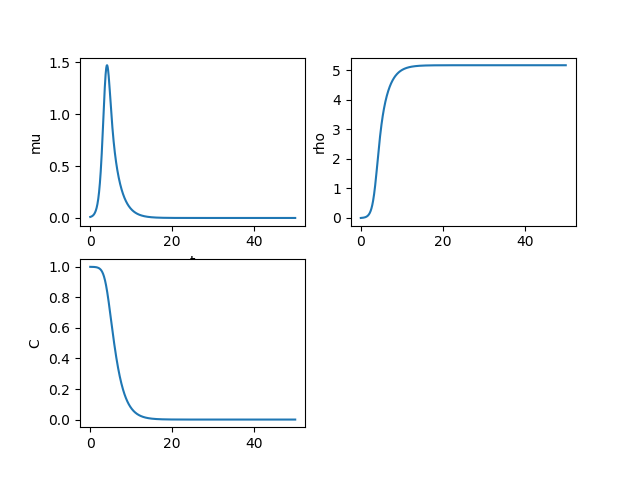
\includegraphics[width=.9\textwidth]{Images/edo_euler_implicite.png}
\caption{Résolution du schéma implicite pour l'EDO}
\end{figure}
 On observe les phénomènes attendus sur l'EDO:\\
 -i) $\mu$ est bornée et tend vers 0.\\
 -ii) $\rho$ est croissante et bornée.\\
 -iii) $C$ décroît vers 0.
\newpage
\subsection{Résolution de l'EDP en 1D}
\subsubsection{Résultat de la simulation de l'EDP en 1D}
\begin{figure}[hbt!]
\centering
\begin{subfigure}[b]{0.45\textwidth}
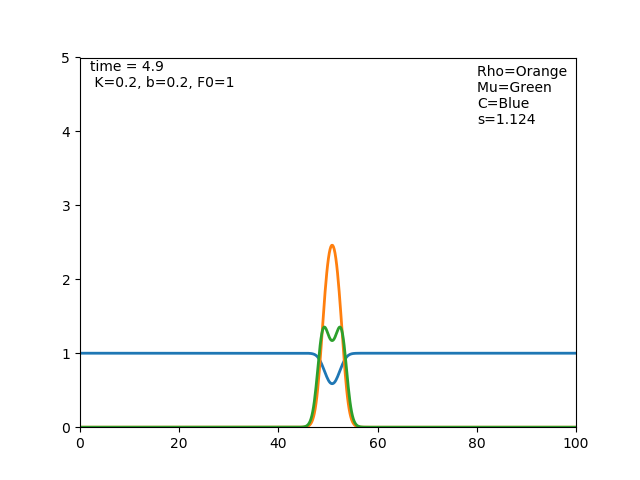
\includegraphics[width=\textwidth]{Images/edp_1d_0.png}
\end{subfigure}
\begin{subfigure}[b]{0.45\textwidth}
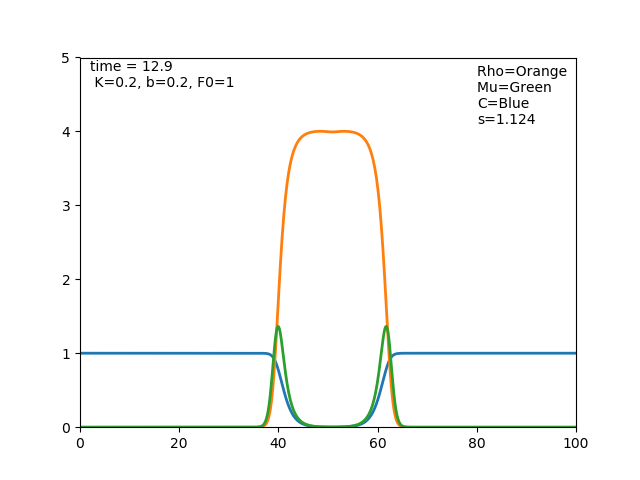
\includegraphics[width=\textwidth]{Images/edp_1d_1.png}
\end{subfigure}
\begin{subfigure}[b]{0.45\textwidth}
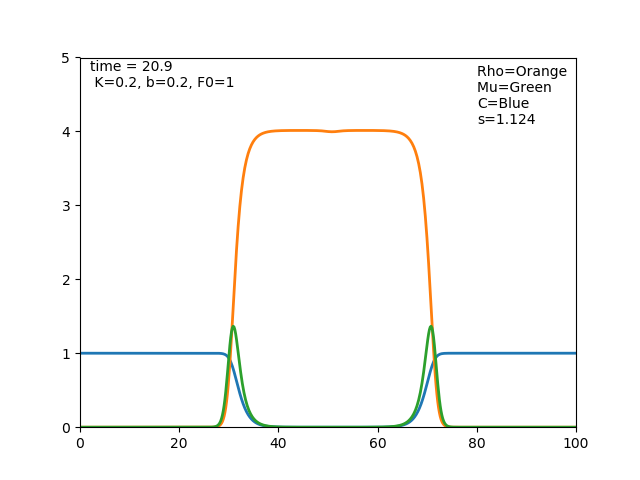
\includegraphics[width=\textwidth]{Images/edp_1d_2.png}
\end{subfigure}
\begin{subfigure}[b]{0.45\textwidth}
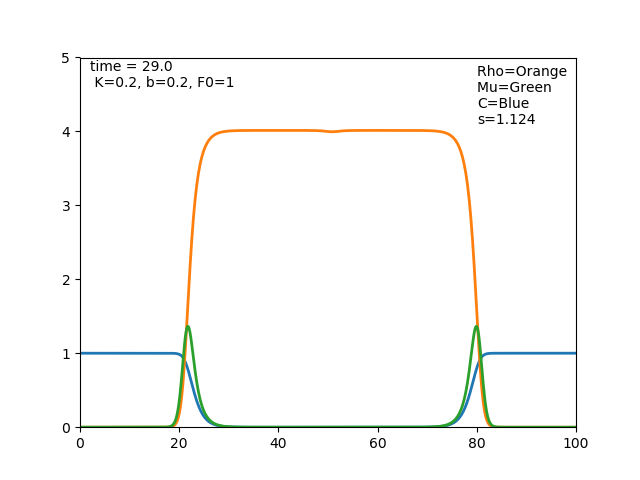
\includegraphics[width=\textwidth]{Images/edp_1d_3.png}
\end{subfigure}
\caption{Résolution du schéma semi implicite I pour l'EDP en 1D} 
\end{figure}
On voit sur les simulations que la solution tend vers une solution de type onde plane stationnaire. Il est possible de calculer cette vitesse et de la comparer avec la vitesse théorique minimale obtenue dans la partie 3: 

\newpage
 
\begin{figure}[hbt!]
\centering
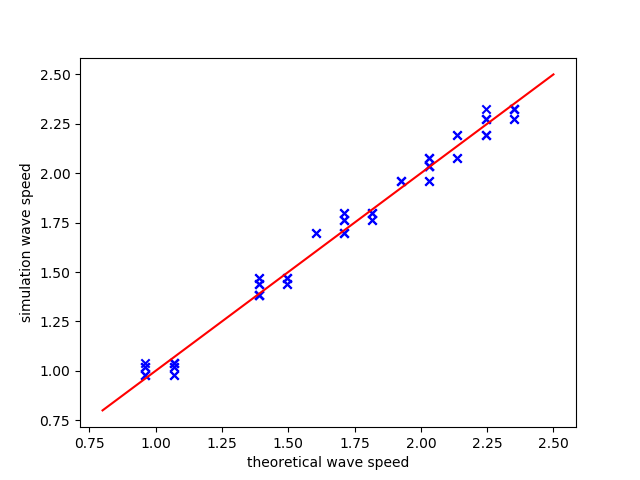
\includegraphics[width=.7\textwidth]{Images/stheoriquevssimulations.png}
\caption{Vitesse du front observée numériquement en fonction de la vitesse minimale théorique}
\end{figure}
Soit \begin{equation*}
s^*_{theorique} =K\frac{f_0(18F_0+4)+\sqrt{f_0(f_0(18F_0+4)^2+108(f_0+4F_0)F_0^2)}}{2(f_0+4F_0)}\end{equation*} la vitesse minimale théorique obtenue dans la partie 3.\\
Ce graphe représente par les points bleus la vitesse du front observée numériquement pour différentes simulations en fonction de la vitesse minimale théorique associée à cette simulation. La droite rouge est la droite $s_{simu} = s^*_{theorique}$.\\
On remarque que la vitesse du front observée numériquement est très proche de la vitesse minimale théorique: ce phénomène est similaire à celui de l'équation de Fisher-KPP: pour une donnée initiale à support compact, \textbf{le front se propage asymptotiquement à la vitesse minimale de l'équation d'onde associée à l'EDP}. %4 et 5
\newpage
\ifdefined\COMPLETE
\else
\documentclass[11pt]{article}
\usepackage[french, english]{babel}
\usepackage[utf8]{inputenc}
\usepackage{graphicx}
\usepackage{framed}
\usepackage[normalem]{ulem}
\usepackage{amsmath}
\usepackage{amsthm}
\usepackage{amssymb}
\usepackage{amsfonts}
\usepackage{enumerate}
\usepackage{import}
\usepackage[top=1 in,bottom=1in, left=1 in, right=1 in]{geometry}
\usepackage{listingsutf8}
\usepackage{color}
\usepackage{float}
\usepackage{graphicx}
\usepackage{subcaption}
\usepackage[toc,page]{appendix}
\usepackage{multicol}
\usepackage{wrapfig}
\usepackage{sidecap}

\floatstyle{boxed} 
\restylefloat{figure}
\definecolor{mygreen}{rgb}{0,0.6,0}
\definecolor{mygray}{rgb}{0.5,0.5,0.5}
\definecolor{mymauve}{rgb}{0.58,0,0.82}
\newcommand{\dt}{\partial_t}
\newcommand{\Tl}{\frac{T}{\lambda}}
\theoremstyle{definition}
\newtheorem{definition}{Définition}[section]
\DeclareMathOperator*{\argmax}{arg\,max}
\DeclareMathOperator*{\argmin}{arg\,min}
 


\lstset{ 
  backgroundcolor=\color{white},   % choose the background color; you must add \usepackage{color} or \usepackage{xcolor}; should come as last argument
  basicstyle=\footnotesize,        % the size of the fonts that are used for the code
  breakatwhitespace=false,         % sets if automatic breaks should only happen at whitespace
  breaklines=true,                 % sets automatic line breaking
  captionpos=b,                    % sets the caption-position to bottom
  commentstyle=\color{mygreen},    % comment style
  deletekeywords={...},            % if you want to delete keywords from the given language
  escapeinside={\%*}{*)},          % if you want to add LaTeX within your code
  extendedchars=true,              % lets you use non-ASCII characters; for 8-bits encodings only, does not work with UTF-8
  firstnumber=1000,                % start line enumeration with line 1000
  frame=single,	                   % adds a frame around the code
  keepspaces=true,                 % keeps spaces in text, useful for keeping indentation of code (possibly needs columns=flexible)
  keywordstyle=\color{blue},       % keyword style
  language=Python,                 % the language of the code
  morekeywords={*,...},            % if you want to add more keywords to the set
  numbers=left,                    % where to put the line-numbers; possible values are (none, left, right)
  numbersep=5pt,                   % how far the line-numbers are from the code
  numberstyle=\tiny\color{mygray}, % the style that is used for the line-numbers
  rulecolor=\color{black},         % if not set, the frame-color may be changed on line-breaks within not-black text (e.g. comments (green here))
  showspaces=false,                % show spaces everywhere adding particular underscores; it overrides 'showstringspaces'
  showstringspaces=false,          % underline spaces within strings only
  showtabs=false,                  % show tabs within strings adding particular underscores
  stepnumber=2,                    % the step between two line-numbers. If it's 1, each line will be numbered
  stringstyle=\color{mymauve},     % string literal style
  tabsize=2,	                   % sets default tabsize to 2 spaces
  title=\lstname                   % show the filename of files included with \lstinputlisting; also try caption instead of title
}
\lstset{inputencoding=utf8/latin1}
\newcommand{\Dt}{\Delta t}
\newcommand{\Dx}{\Delta x}
 %file containing all the used libraries
\begin{document}
\fi


\section{Appendices}
\subsection{Code de résolution de l'EDO}
\lstinputlisting[language=Python]{edo.py}
\newpage
\subsection{Code de la résolution de l'EDP en 1D}
\lstinputlisting[language=Python]{edp_1d.py}
\newpage
\subsection{Code de la résolution de l'EDP en 2D}
\lstinputlisting[language=Python]{edp_2d.py}

\ifdefined\COMPLETE
\else
\end{document}
\fi

\end{document}